\documentclass[../../script.tex]{subfiles}
% !TEX root = ../../script.tex

\begin{document}
\section{Convergence of Function sequences}

\begin{defi}[Pointwise convergence]
    Let $M$ be a set, $f_n: M \rightarrow \field ~~\forall n \in \natn$ and $f: M \rightarrow \field$. 
    The sequence $\seq{f}$ is said to be pointwise convergent to $f$ if 
    \[
        \limn f_n(x) = f(x) ~~\forall x \in M
    \]
\end{defi}

\begin{eg}
    Consider
    \begin{align*}
        f_n: [0, 1] &\longrightarrow \realn \\
        x &\longmapsto \begin{cases}
            1 - nx, & x \in [0, \frac{1}{n}] \\
            0, & \text{else}
        \end{cases}
    \end{align*}

    \begin{center}
        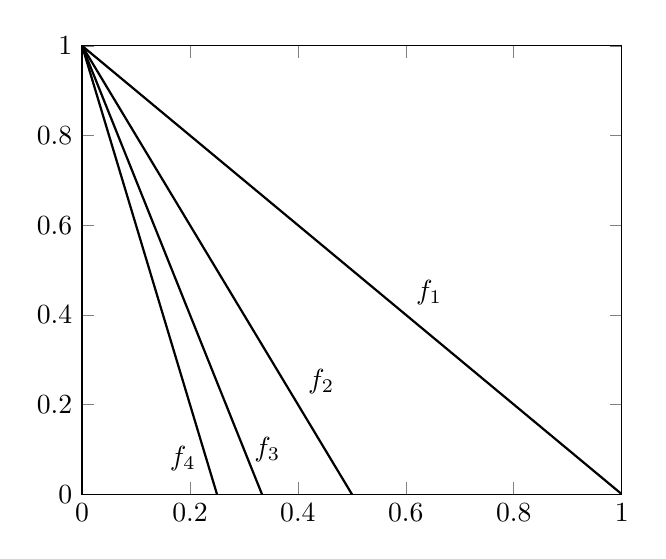
\begin{tikzpicture}[domain=0:1]
            \begin{axis}[xmin=0, ymin=0, xmax=1, ymax=1, samples=50]
                \addplot[black, thick] {1-x} node[above right, pos=0.6] {$f_1$};
                \addplot[black, thick] {1-2*x} node[above right, pos=0.4] {$f_2$};
                \addplot[black, thick] {1-3*x} node[right, pos=0.3] {$f_3$};
                \addplot[black, thick] {1-4*x} node[left, pos=0.23] {$f_4$};
            \end{axis}
        \end{tikzpicture}
    \end{center}
    The $f_n$ are continuous for all $n \in \natn$ and converge pointwise to 
    \begin{align*}
        f: [0, 1] &\longrightarrow \realn \\
        x &\longmapsto \begin{cases}
            1, & x = 0 \\
            0, & x \ne 0
        \end{cases}
    \end{align*}
    $f$ is not continuous.
\end{eg}

\begin{rem}
    Let $M$ be a set. Then 
    \[
        B(M) = \set[\exists K \in \realn: ~~|f(x)| < K ~~\forall x \in M]{f_n: M \longrightarrow \field}
    \]
    is a linear subspace of the space of all functions $M \rightarrow \field$. We can define the supremum norm 
    \begin{align*}
        \supnorm{\cdot}: B(M) &\longrightarrow \realn \\
        f &\longmapsto \sup_{x \in M}\set{\abs{f(x)}}
    \end{align*}
\end{rem}
\begin{proof}
    We will now proof that $\supnorm{\cdot}$ is a norm. 
    It is defined, because 
    \begin{equation}
        \supnorm{f} = 0 \implies \abs{f(x)} = 0 ~~\forall x \in M
    \end{equation}
    This implies 
    \begin{equation}
        f(x) = 0 ~~\forall x \in M \implies f = 0
    \end{equation}
    The triangle inequality is proven by first considering
    \begin{equation}
        \abs{f(x)} \le \supnorm{f} ~~\forall f \in B(M) ~\forall x \in M
    \end{equation}
    Let $f, g \in B(M)$, then 
    \begin{equation}
        \abs{f(x) + g(x)} \le \abs{f(x)} + \abs{g(x)} \le \supnorm{f} + \supnorm{g} ~~\forall x \in M
    \end{equation}
    Which implies 
    \begin{equation}
        \supnorm{f + g} = \sup_{x \in M} \abs{f(x) + g(x)} \le \supnorm{f} + \supnorm{g}
    \end{equation}
\end{proof}

\begin{defi}[Uniform convergence]
    A sequence of bounded functions $\seq{f}$,
    \[
        f_n: M \longrightarrow \field
    \]
    is said to be uniformly convergent to $f: M \rightarrow \field$ if its norm converges.
    \[
        \supnorm{f_n - f} \conv{n \rightarrow \infty} 0
    \]
\end{defi}

\begin{rem}
    Formally, pointwise convergence means 
    \[
        \forall \epsilon > 0 ~\forall x \in M ~\exists N \in \natn ~\forall n \ge N: ~~\abs{f_n(x) - f(x)} < \epsilon
    \]
    and uniform convergence means 
    \[
        \forall \epsilon > 0 ~\exists N \in \natn ~\forall x \in M ~\forall n \ge N: ~~\abs{f_n(x) - f(x)} < \epsilon
    \]
\end{rem}

\begin{thm}
    The function space $B(M)$ is complete.
\end{thm}
\begin{proof}
    Let $\anyseqdef[f]{B(M)}$ be a Cauchy sequence in terms of $\supnorm{\cdot}$. Firstly, we have for some fixed $x \in M$
    \begin{equation}
        \abs{f_n(x) - f_m(x)} \le \supnorm{f_n - f_m}
    \end{equation}
    Since $\seq{f}$ is a Cauchy sequence, $(f_n(x))$ is also a Cauchy sequence in $\field_0$. Because $\field$ is complete,
    $(f_n(x))$ converges, and we define 
    \begin{equation}
        f(x) = \limn f_n(x)
    \end{equation}
    thus $\seq{f}$ converges pointwise to $f$. Let $\epsilon > 0$. Then 
    \begin{equation}
        \exists N \in \natn: ~~\supnorm{f_n \cdot f_m} < \epsilon ~~\forall n, m \ge N
    \end{equation}
    Then $\forall x \in M, ~\forall n, m \ge N$ we have 
    \begin{equation}
        \abs{f_n(x) - f_m(x)} \le \supnorm{f_n - f_m} < \epsilon
    \end{equation}
    We can find the limit for $m \rightarrow \infty$
    \begin{equation}
        \abs{f(x) - f_n(x)} \le \epsilon
    \end{equation}
    and 
    \begin{equation}
        \supnorm{f} = \sup_{x \in M}\abs{f} \le \sup_{x \in M} \abs{f(x) - f_n(x)} + \sup_{x \in M} \abs{f_n(x)} = \epsilon + \supnorm{f_n}
    \end{equation}
    Thus, $f$ is bounded. Furthermore
    \begin{equation}
        \supnorm{f - f_n} = \sup_{x \in M} \abs{f(x) - f_n(x)} \le \epsilon
    \end{equation}
    which in turn implies 
    \begin{equation}
        \supnorm{f - f_n} \conv{n \rightarrow \infty} 0
    \end{equation}
\end{proof}

\begin{defi}
    Let $\metric$ be a metric space, then $C_b(X)$ is said to be the space of all continuous bounded functions.
\end{defi}

\begin{rem}
    If $X$ is compact (e.g. a bounded, closed subset of $\realn^n$) then all continuous functions are bounded. We then write $C(X)$ for $C_b(X)$.
\end{rem}

\begin{thm}
    Let $\metric$ be a metric space. $C_b(X)$ is closed in $B(X)$. In other words, every uniformly convergent sequence of continuous functions converges to a continuous function.
\end{thm}
\begin{proof}
    Let $\anyseqdef[f]{C_b(X)}$ be a sequence that uniformly converges to $f \in B(X)$. 
    Let $x \in X$ and $\epsilon > 0$, then 
    \begin{equation}
        \exists N \in \natn: ~~\supnorm{f - f_n} y \frac{\epsilon}{3} ~~\forall n \ge N
    \end{equation}
    Choose a fixed $n \ge N$. Since $f_n$ is continuous, this means that 
    \begin{equation}
        \exists \delta > 0: ~~\abs{f_n(x) - f_n(y)} < \frac{\epsilon}{3} ~~\forall y \in \oball[\delta](x)
    \end{equation}
    Then we have for all such $y$
    \begin{equation}
        \begin{split}
            \abs{f(x) - f(y)} &\le \abs{f(x) - f_n(x)} + \abs{f_n(x) - f_n(y)} + \abs{f_n(y) - f(y)} \\
            &\le 2 \cdot \supnorm{f - f_n} + f_n(x) - f_n(y) < \epsilon
        \end{split}
    \end{equation}
    This proves the continuity of $f$ in $x$. Since $x \in X$ was chosen arbitrarily, $f$ is continuous everywhere.
\end{proof}

\begin{defi}
    Let $x_0 \in \field$ and $\anyseqdef[a]{\field}$. Then 
    \[
        \series{n} a_n (x - x_0)^n
    \]
    is called a power series around $x_0$. The number 
    \[
        \rho := \sup\set[\series{n} a_n (x - x_0)^n \text{ converges}]{\abs{x - x_0}}
    \]
    is the convergence radius.

    \begin{center}
        \begin{tikzpicture}
            \draw[->, thick] (0, 0) -- (0, 4) node [above] {};
            \draw[->, thick] (0, 0) -- (4, 0) node [right] {};
            
            \draw[fill] (2, 2) circle [radius=1pt] node [below right] {$x_0$};
            \draw[dashed] (2, 2) circle [radius=1.2cm];

            \draw[<->, rotate around={45:(2, 2)}] (2, 2) -- node[above] {$\rho$} (3.2, 2);

            \draw[fill, rotate around={100:(2, 2)}] (3.2, 2) circle [radius=1pt] node [above] {$x$};
        \end{tikzpicture}
    \end{center}
\end{defi}

\begin{rem}
    All results so far (including proofs) can be extended to $\realn^n$-valued functions, or functions with values in a Banach space in general.
\end{rem}

\begin{thm}
    Let $\series{n} a_n (x - x_0)^n$ be a power series with convergence radius $\rho \in [0, \infty) \cup \set{\infty}$.
    If $\abs{x - x_0} < \rho$ then the series converges absolutely, for $\abs{x - x_0} > \rho$ it diverges.
    \[
        \frac{1}{\rho} = \limsupn \sqrt[n]{\abs{a_n}}
    \]
\end{thm}
\begin{proof}
    W.l.o.g. choose $x_0 = 0$:
    For $\abs{x} > \rho$ the series diverges by definition. If $\abs{x} < \rho$ then there exists $y \in \field$ such that
    $\abs{x} < \abs{y} \le \rho$ and $\series{n} a_n y^n$ convergent. Especially, $(a_n y^n)$ is a null sequence.
    This means $\exists C > 0$ such that $\abs{a_n y^n} \le C ~~\forall n \in \natn$
    \begin{equation}
        \series{n} \abs{a_n x^n} = \series{n} \abs{a_n y^n} \abs{\frac{x}{y}}^n \le C \cdot \series{n} \abs{\frac{x}{y}}^n < \infty
    \end{equation}
    This statement only holds for $\rho > 0$.
\end{proof}

\begin{rem}
    \begin{enumerate}[(i)]
        \item We have 
        \[
            \rho = \sup \set[\series{n}\abs{a_n}a^n \text{ converges}]{a \in [0, \infty)}
        \]

        \item If the following limit exists, then 
        \[
            \rho = \limn \frac{\abs{a_n}}{\abs{a_{n+1}}}
        \]
    \end{enumerate}
\end{rem}

\begin{eg}
    The series 
    \[
        \series{n} x^n
    \]
    is convergent on $(-1, 1)$, so $\rho = 1$. The limit function is 
    \[
        x \longmapsto \frac{1}{1 - x}
    \]
\end{eg}

\begin{thm}
    Let $\series{n} a_n (x - x_0)^n$ be a power series with convergence radius $\rho > 0$. 
    Let $0 < a < \rho$. Then this power series converges uniformly on $\cball[a](x_0)$. Especially
    \begin{align*}
        f: \oball[\rho](x_0) &\longrightarrow \realn \\
        x &\longmapsto \series{n} a_n (x_n - x_0)^n
    \end{align*}
\end{thm}
\begin{proof}
    W.l.o.g. choose $x_0 = 0$. Let $0 < a < \rho$. We know that $\series{n} a_nx^n$ converges on $\cball[a](0)$. 
    
    \begin{center}
        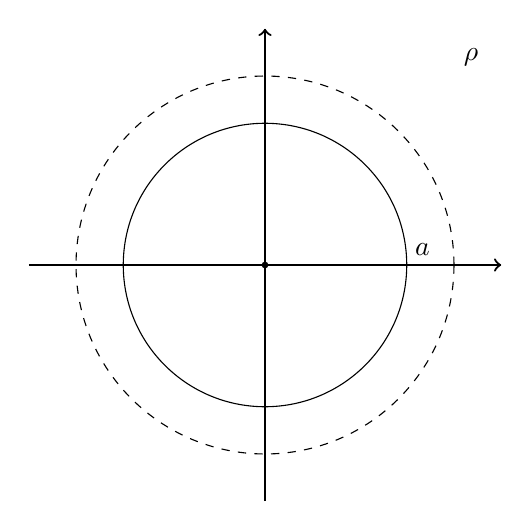
\begin{tikzpicture}
            \draw[->, thick] (0, -3) -- (0, 3);
            \draw[->, thick] (-3, 0) -- (3, 0);

            \draw[fill] (0, 0) circle [radius=1pt];

            \draw[solid] (0, 0) circle [radius=1.8cm];
            \draw[dashed] (0, 0) circle [radius= 2.4cm] node[above right=2.4cm] {$\rho$};

            \node at (2, 0.2) {$a$};
        \end{tikzpicture}
    \end{center}

    Define 
    \begin{equation}
    \begin{split}
        f_n: \cball[a](0) &\longrightarrow \field \\
        x &\longmapsto x^n ~~\forall n \in \natn
    \end{split}
    \end{equation}
    We can see that 
    \begin{equation}
        \supnorm{f} = \sup_{x \in \cball[a](0)} \abs{f_n} = \sup_{x \in \cball[a](0)} = a^n
    \end{equation}
    and thus 
    \begin{equation}
        \series{n} a_n f_n \implies \series{n} \supnorm{a_n f_n} = \series{n} \abs{a_n}^n < \infty
    \end{equation}
    because $a < \rho$. The series $\series{n} a_n f_n$ is absolutely convergent in $C(\cball[a](0))$.
    Since $C(\cball[a](0))$ is complete, $\series{n} a_n f_n$ is convergent because the partial sums $\series[N]{n} a_n f_n$ are continuous $\forall N \in \natn$.
    Therefore $f$ is also continuous on $\cball[a](0)$. Let $x \in \oball[\rho](0)$. Then there exists some $a > 0$ such that $\abs{x} < a < \rho$.
    Thus, $f$ is continuous on $\cball[a](0)$. Since $\cball[a](0)$ contains a neighbourhood of $x$, and continuity is a local property,
    $f$ is also continuous in $x$. Because $x \in \oball[\rho](0)$ was chosen arbitrarily, $f$ is continuous.
\end{proof}

\begin{rem}
    $\exp$, $\sin$, $\cos$ are continuous.
\end{rem}

\begin{eg}
    The statements above can be extended to Banach space-valued power series (e.g. matrix-valued functions).
    The norm on $\realn^{n \times n}$ is 
    \[
        \norm{A} = \sup\set[{\forall x \in \oball[1](0)}]{\norm{Ax}}
    \]
    Define 
    \[
        \exp(A) := \series{0} \frac{A^n}{n!}
    \]
    This converges $\forall A \in \realn^{n \times n}$, because
    \begin{align*}
        \series{n} \norm{\frac{A^n}{n!}} &= \series{n} \frac{1}{n!} \norm{A^n} \le \series{n} \frac{1}{n!} \norm{A}^n \\
        &= \exp(\norm{A}) < \infty
    \end{align*}
    Thus, $\series{n} \frac{A^n}{n!}$ converges absolutely. Now consider the function 
    \begin{align*}
        \realn &\longrightarrow \realn^{n \times n} \\
        t &\longmapsto \exp(At)
    \end{align*}
    This is a matrix-valued power series
    \[
        \exp(At) = \series{n} \frac{(At)^n}{n!} = \series{n} \frac{A^n}{n!} t^n
    \]
    with a convergence radius of $\rho = \infty$. In this case $\exp(A + B)$ doesn't necessarily have to equal $\exp(A) \cdot \exp(B)$.
\end{eg}
\end{document}